%%%%%%%%%%%%%%%%%%%%%%%%%%%%%%%%%%%%%%%%%
% Thin Sectioned Essay
% LaTeX Template
% Version 1.0 (3/8/13)
%
% This template has been downloaded from:
% http://www.LaTeXTemplates.com
%
% Original Author:
% Nicolas Diaz (nsdiaz@uc.cl) with extensive modifications by:
% Vel (vel@latextemplates.com)
%
% License:
% CC BY-NC-SA 3.0 (http://creativecommons.org/licenses/by-nc-sa/3.0/)
%
%%%%%%%%%%%%%%%%%%%%%%%%%%%%%%%%%%%%%%%%%

%----------------------------------------------------------------------------------------
%   PACKAGES AND OTHER DOCUMENT CONFIGURATIONS
%----------------------------------------------------------------------------------------

\documentclass[a4paper, 11pt]{article} % Font size (can be 10pt, 11pt or 12pt) and paper size (remove a4paper for US letter paper)

\usepackage{hyperref}
\usepackage[portuguese,english]{babel}
\usepackage[utf8]{inputenc}
\usepackage{float}

\usepackage{color} % for the notes
\usepackage{xcolor}
\usepackage[protrusion=true,expansion=true]{microtype} % Better typography
\usepackage{graphicx} % Required for including pictures
\usepackage{wrapfig} % Allows in-line images
\usepackage{tocloft}
\usepackage{multirow}

\usepackage{mathpazo} % Use the Palatino font
\usepackage[T1]{fontenc} % Required for accented characters
\linespread{1.05} % Change line spacing here, Palatino benefits from a slight increase by default
\usepackage{etoolbox}
\newcommand{\githubi}{Git\textsc{h}ub}
\newcommand{\bdoh}{{\sc b}lack {\sc d}uck {\sc o}pen \textsc{hub}}
\newcommand{\ohloh}{\textsc{o}hloh}
\newcommand{\php}{\textsc{php}}
\newcommand{\twitter}{\textsc{t}witter}
\newcommand{\facebook}{\textsc{f}acebook}
\newcommand{\msn}{\textsc{msn}}
\newcommand{\gchat}{\textsc{g}oogle \textsc{c}hat}
\newcommand{\bash}{\textsc{b}ash}
\newcommand{\python}{\textsc{p}ython}
\newcommand{\django}{\textsc{d}jango}
\newcommand{\curl}{c\textsc{url}}
\newcommand{\firefox}{\textsc{f}irefox}
\newcommand{\floss}{\textsc{floss}}
\newcommand{\openoffice}{\textsc{o}pen\textsc{o}ffice}
\newcommand{\puredata}{\textsc{p}uredata}
\newcommand{\schema}{\textsc{s}chema.org}
\newcommand{\wiki}{\textsc{w}iki}
\newcommand{\nosql}{\textsc{n}o\textsc{sql}}
\newcommand{\etherpad}{\textsc{e}therpad}
\newcommand{\irc}{\textsc{irc}}
\newcommand{\irci}{\textsc{Irc}}
\newcommand{\ocd}{\textsc{ocd}}
\newcommand{\participa}{\textsc{p}articipa.br}
\newcommand{\httpb}{\textsc{http}}
\newcommand{\foaf}{\textsc{foaf}}
\newcommand{\ops}{\textsc{ops}}
\newcommand{\sioc}{\textsc{sioc}}
\newcommand{\gndo}{\textsc{gndo}}
\newcommand{\html}{\textsc{html}}
\newcommand{\ggg}{\textsc{ggg}}
\newcommand{\opa}{\textsc{opa}}
\newcommand{\obs}{\textsc{obs}}
\newcommand{\vbs}{\textsc{vbs}}
\newcommand{\lod}{\textsc{lod}}
\newcommand{\nlp}{\textsc{nlp}}
\newcommand{\sectionb}{\textsc{s}ection}
\newcommand{\cn}{\textsc{cn}}
\newcommand{\aab}{\textsc{aa}}
\newcommand{\dc}{\textsc{d}ublin {\sc c}ore}
\newcommand{\json}{\textsc{json}}
\newcommand{\flask}{\textsc{f}lask}
\newcommand{\aai}{\textsc{Aa}}
\newcommand{\ontologiaa}{\textsc{o}ntologi\textsc{aa}}
\newcommand{\ontologiaai}{\textsc{O}ntologi\textsc{aa}}
\newcommand{\owl}{{\sc owl}}
\newcommand{\www}{{\sc www}}
\newcommand{\rdfi}{{\sc Rdf}}
\newcommand{\mongodb}{{\sc m}ongo{\sc db}}
\newcommand{\mysql}{{\sc m}y{\sc sql}}
\newcommand{\rdf}{{\sc rdf}}
%\newcommand{\paaineli}{P{\sc aa}inel}
\newcommand{\paaineli}{P{\bf \sc aa}inel}
\newcommand{\paainel}{p{\sc aa}inel}
\newcommand{\gsd}{\textsc{gsd}}
\newcommand{\ui}{\textsc{ui}}
%\newcommand{\lmb}{\url{lab\textsc{M}acambira.sf.net}}
\newcommand{\lm}{lab\textsc{M}acambira.sf.net}
%\newcommand{\lm}{\url{labMacambira.sf.net}}



\makeatletter
\renewcommand\@biblabel[1]{\textbf{#1.}} % Change the square brackets for each bibliography item from '[1]' to '1.'
\renewcommand{\@listI}{\itemsep=0pt} % Reduce the space between items in the itemize and enumerate environments and the bibliography

\hypersetup{
        colorlinks,
            linkcolor={red!50!black},
                citecolor={blue!50!black},
                    urlcolor={blue!80!black}
                }


\pretocmd{\chapter}{\addtocontents{toc}{\protect\addvspace{5\p@}}}{}{}
\pretocmd{\section}{\addtocontents{toc}{\protect\vspace{-4mm}}}{}{}
\renewcommand{\maketitle}{ % Customize the title - do not edit title and author name here, see the TITLE block below
\begin{flushright} % Right align
{\LARGE\@title} % Increase the font size of the title

\vspace{50pt} % Some vertical space between the title and author name

{\large\@author} % Author name
\\\@date % Date

\vspace{40pt} % Some vertical space between the author block and abstract
\end{flushright}
}

%----------------------------------------------------------------------------------------
%   TITLE
%----------------------------------------------------------------------------------------

\title{\textbf{The Algorithmic-Autoregulation essay}\\ % Title
%a natural collective focus\\on the collective being} % Subtitle
a collective and natural focus\\ on self-transparency} % Subtitle

\author{\textsc{Renato Fabbri} % Author
\\{\textit{IFSC/USP, Participa.br/SG-PR, labMacambira.sf.net}}} % Institution

\date{\today} % Date

%----------------------------------------------------------------------------------------

\begin{document}

\maketitle % Print the title section

%----------------------------------------------------------------------------------------
%   ABSTRACT AND KEYWORDS
%----------------------------------------------------------------------------------------

%\renewcommand{\abstractname}{Summary} % Uncomment to change the name of the abstract to something else


\begin{abstract}
    There are numerous pursues for a lightweight and systematic account of what is done by a group and containing individuals. The Algorithmic-Autoregulation (\aab) is a special case, in which a technical community embraced the challenge of registering their own dedication for sharing processes, self-transparency enhancements, and prove dedication. \aai\ is used since June/2011 by dozens of \floss\ and social developers, with the support of different \aab\ software gadgets and for distinct tasks. Intermittence and activity concentration of users activity follows expected natural properties. Social participation and ontological understandings of \aab\ eases comparative analysis and furthers integration.
\end{abstract}

{
\selectlanguage{portuguese}
\begin{abstract}

\end{abstract}
}

\hspace*{3,6mm}\textit{Keywords:} distributed development, \floss, social participation, \owl, statistics, anthropological physics % Keywords

%\vspace{30pt} % Some vertical space between the abstract and first section

%----------------------------------------------------------------------------------------
%   ESSAY BODY
%----------------------------------------------------------------------------------------
\newpage
\tableofcontents


\section{\aai\ concept}\label{sec:start}
%\addcontentsline{toc}{section}{\aai\ start}
The Algorithmic Autoregulation (\aab) is a self-transparency mechanism for sharing processes, proving dedication, and enhance personal or collective self-transparency. Purposes for \aab\ usage are numerous: enable automated and fair compensation for dedications, ease co-working, introduce newcomers, keeping public historical logs of activities, etc. Indeed, other systems have been designed for such a task (see Section~\ref{sec:rel}). A brief characterization of \aab\ is:
\begin{itemize}
    \item The collective origin, purpose and upkeep. This is a free-culture trait, present within many software, and leads to open software and data as described in Section ~\ref{sec:sofsup}.
    \item Voluntary logging of messages about ongoing work.
    \item Enables coordinating distributed team work through individual merit.
    \item More a practice than a software: \aab\ presents variations on the software support and message composition. Often present features are screencasts, peer validation and periodic messaging.
\end{itemize}

Transparency in this context should be understood as usual organization or State transparency is: a public account of activities~\cite{stso}; not directly as transparency in self-knowledge, as is the case in some philosophical and political contexts~\cite{stph}. One should reach~\cite{paaper} for a noteworthy overview of \aab\ as a Global Software Development (\gsd).

 \subsection{Related work}\label{sec:rel}
%\addcontentsline{toc}{subsection}{Related work}
 Authors know of no \emph{civil society transparency} platform. There is a number of transparency initiatives for governments~\cite{govTr}, for religious parties~\cite{espTr} and for private institutions~\cite{priTr}. Data analysis methods are derived from Natural Language Processing (\nlp) and Complex Networks (\cn) fields, constituting a hybrid framework of classical~\cite{cla1,cla2} and novel~\cite{nov1,nov2} approaches.

\subsection{Historical note}
7th June, 2013, Cleodon Silva~\cite{cleodon} died by heart failure. In his memory, the \lm\ group was born (Pedro Macambira was one of this pseudonyms). The \aab\ was conceived as the ``cardiac pulse'' of the group and is in constant usage since July, 2011. It gathers thousands of messages, tenths of users and hundreds of processes. \aai\ messages present contributions, such as  commits to official repositories of Evince, \firefox, \openoffice, \puredata\ and other software~\cite{paaper}. A number of other activities were registered: new software elaboration and coding, writing of articles, \wiki s and \etherpad s; articulation of civil society, academic and state instances; studies and reviews. Even so, \aab\ is highly biased towards software development, as can be observed in \sectionb s~\ref{sec:stats} and~\ref{sec:res}, and in the \gsd\ article about \aab~\cite{paaper}.

\subsection{Essay structure}\label{sec:ess}
Section~\ref{sec:use} describes \aab\ uses incident and envisioned.
Section~\ref{sec:sofsup} exposes different software written or used for \aab. Section~\ref{sec:data} is dedicated to data. Section~\ref{sec:stats} further develops statistics about \aab\ in terms of vocabulary and networks. Section~\ref{sec:res} states results and \sectionb~\ref{sec:con} a concludes with further works and acknowledgements. Tables and figures are inplace, kept as simple briefings and illustrations. External resources - mainly documents, data and scripts - are referenced for further inspection.

\section{Design features}\label{sec:desf}
To understand use practices and software support (\sectionb s~\ref{sec:use} and~\ref{sec:sofsup}), one needs to observe core design features of \aab:
\begin{itemize}
    \item Evenly spaced messages should be sent by the \aab\ user. The time lapse is called a ``slot'' and the message a ``shout''. A slot might refer to the time lapse and the message, this is context dependent and will be pointed on text if ambiguity occurs.
    \item Shouts should report the task being tackled and/or a briefing of what was done in the slot.
    \item Shouts are grouped into ``sessions''. Each session is ideally linked with a short screencast by the user, with a few dozen seconds of explanation about the \aab\ session.
    \item Each session is sent by email to a random \aab\ user for validation.
\end{itemize}

Variants of this features were conceived and practiced. Figure~\ref{fig:consult} exposes a diagram shared and referenced by \aab\ users in the first months of \aab\ practice.


\begin{figure}[!h]
    \centering
    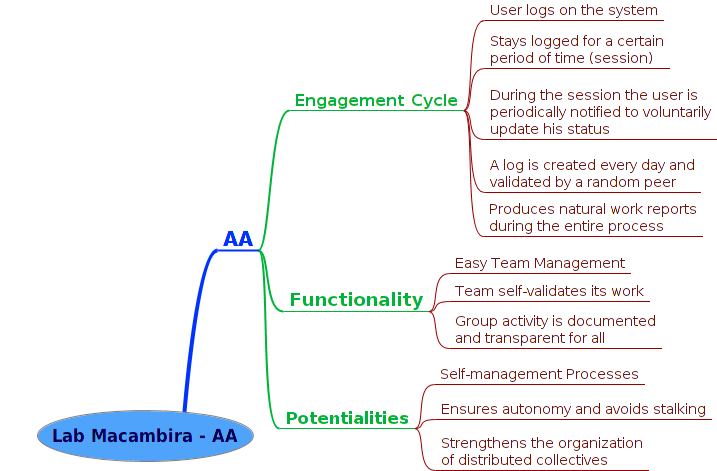
\includegraphics[width=\textwidth]{imgs/aaFirstMethodology}
    \caption{A mind map of the AA methodology shared by users: i) Engagement cycle – the usage of AA; ii) Functionality – the design goals of the system; iii) Potentialities – envisioned benefits of AA by authors of the diagram. As seen in Section~\ref{sec:start}, core benefits emanate from the self-transparency aspect of~\aab, with worthy mentions to proving dedications and sharing processes.} 
    \label{fig:consult}
\end{figure}




\section{Use practices}\label{sec:use}
%\addcontentsline{toc}{subsection}{Systematic use proposals}
%tags, slots, spacing, scattered, etc. Offline
Distinct use methods are incident, mostly regarding the design exposed in \sectionb~\ref{sec:desf}. Even those cases which are not standard can be understood in the light of \aab\ paradigm. Deviations from the ideal case is always present (\sectionb~\ref{sec:devia}).

\subsection{Words and tags}\label{sec:usewt}
Throughout \aab\ usage, particular words and tags has been used to classify shouts. Of particular interest are:
\begin{itemize}
    \item Hashtags, such as \#aa, \#coding and \#articulation. These were inherited from Twitter practice. 
    \item Tags starting with ``+'' sign, such as +django, +sna and +reading. These aimed at particular used of tagging within \aab, with independence of other systems and easing concurrent use of \aab\ and other social networks.
    \item Words and abbreviations. Sometimes used in the beginning of shouts, others on the end of them, these also had the purpose of easing categorization of the shouts. These cases sometimes were pointed as tags for entire sessions or for all shouts since tagging, until another tagging shout was sent by the user.
\end{itemize}

These tagging schemes was also used as a way to enable the ``ubiquitous \aab'', i.e. usage of \aab\ in any social network or communication protocol. The \#aao0 tag was used for Twitter streaming \aab\ shouts to a considered database as is the most prominent ubiquitous \aab\ manifestation. Facebook tagging was also used to indicate posts and comments that were \aab\ shouts. On some extreme cases, tagging was used in any platform, considering ubiquitous \aab\ implemented, but not yet mined.

\subsection{Messages}\label{sec:usesh}
Messages for \aab\ usage can be of various types, as shown in Table~\ref{tab:msgTy}. Usually, the type was dictated by first word of the message. Start messages started an \aab\ session, while stop messages finished an ongoing session. Push messages sent local \aab\ sessions (or independent shouts) to a shared database. There was only one automatic message, designated to register ``lost timeslot'' of sessions (see Section~\ref{sec:usess}). Additional messages were dedicated to query for tickets attributed to the user, milestones and other traditional software development managements facilities.

\subsubsection{Shouts}
By far the most important \aab\ related message to date is the ``shout''. Dedicated to expose ongoing tasks, shouts are recurrently envisioned as a structured message, in which the user classifies the shout through special words and tags, and describes ongoing efforts with natural language (usually Portuguese or English). Example of structured shout proposals are in~\cite{aaWiki} and~\cite{aaREADME}. Nevertheless, shouts are used by all \aab\ users, in almost all cases, without such sophisticated structure, but as a plain short natural language description of current efforts, i.e. without classification whatsoever of the message. 

\subsection{Sessions}\label{sec:usess}
\aai\ sessions are collections of \aab\ shouts.
These have had incidence in \aab\ practice:
\begin{itemize}
    \item Shouts within a session were input by user each 15 minutes.
    \item Tolerance for shouts in an ideal session was of $\pm 5$ minutes, considered 15 minutes grid.
    \item Total duration of 2h, in which 8 shouts should outline tasks and technologies.
    \item A short screencast was recorded at the end of each session, in which the user exposed dedication within seconds.
    \item The session was sent to a random user for peer validation in which the session received a score based on shouts and screencast.
\end{itemize}

Such a session design was very important in first 6 months of \aab,
where each of almost 10 apprentices were dedicating a session per day.
Other users also delivered \aab\ sessions, but not as regularly.
Noteworthy: \aab\ shouts can be separated by durations different from 15 minutes: 
example of incident shout separations include 5 minutes, 2 minutes, 30 minutes, 1h.
Most shouts are not explicitly related to sessions, but most shouts still occur in
a session-like context. This is regarded as a consequence of the intuitive usage
\aab\ sessions were aimed for, and as an inheritance of early \aab\ practice.
From now on, \aab\ session is going to be used as meaning both a session registered as such,
as an arbitrary time-contiguous set of shouts from the same user. Text will point such
specificity if necessary.

\subsection{Accomplishments}\label{sec:usedev}
Processes registered by \aab\ usage often purposes to accomplish something: 
write a software or an article;
make images, music or research scripts; 
articulate groups, read technical material or take online classes; etc. 

These tasks usually spread entire sessions. Sometimes, one session can embrace
multiple tasks. A quite common \aab\ usage is to shout one or just a few
messages about current efforts, without much care for regularity or
completeness.

\subsection{Deviations from \aab\ paradigm}\label{sec:devia}
There are at least three perceived deviations from \aab\ paradigm, all most often within new users:
\begin{itemize}
    \item Advertising: shouts containing propaganda about events and groups. This behavior is attributed to both 1) common practice in more commercial platforms, such as Twitter and Facebook; and as 2) the outcome of the \aab\ unusual goals and design, which requires acculturation from a regular visitor before proper understanding.
    \item Final product exhibitionism: shouts containing not ongoing processes, but only a media or deed recently completed. Although not considered entirely wrong by users, it does not accomplish \aab\ mechanism as posed in Section~\ref{sec:start}.
    \item Introduction to \aab, \irc\ and hacking: handling \aab\ is regarded as empowerment and introduction to hacking and open co-working. This first approximation is often marked by playful and test shouts. Although very well esteemed, these messages are also deviations from \aab\ purpose.
\end{itemize}
 \section{Software support}\label{sec:sofsup}
%\addcontentsline{toc}{section}{Systems and data}
 Different software support for \aab\ is exposed in this section. Section~\ref{sec:data} is dedicated to their integration as linked data, both within \aab\ variants and within participatory instances.

There are mainly three software pieces written to support \aab\ activity. Two of them are a server and client suite each (see Sections~\ref{sec:aaFirst} and~\ref{sec:aa01}). The third is a fancy dashboard. Among supplementary software support are an automated conversational agents (software [ro]bots), used as alternative User Interfaces (\ui s), with a highlight for the Lalenia bot (see Section~\ref{sec:lalenia}); and an initiative to make \aab\ available in all chat networks (see Section~\ref{sec:ubi}).

All \aab\ software apparatus is contextualized in Table~\ref{tab:aas}.

\subsection{First \aab: \httpb\ server, \html\ skin and shell client}\label{sec:aaFirst}
Although deprecated in favor of \aab\ 01, this first \aab\ software presents the most numerous set of functionalities. Client was completely designed for GNU/Linux terminal usage, and the  functionalities are:
\begin{itemize}
    \item Sending messages to the host.
    \item Configuration facilities.
    \item Access to tickets and other software developments facilities.
    \item Timing to ease \aab\ usage, as described in Sessions~\ref{sec:desf} and~\ref{sec:usess}.
\end{itemize}

Server functionalities are:
\begin{itemize}
    \item Receiving shouts and other \aab\ messages through \httpb.
    \item Registering shouts and other \aab\ messages, received through \httpb, in a \mysql\ database.
\end{itemize}

Core \html\ skin functionalities are:
\begin{itemize}
    \item Exhibiting shouts and sessions to other \aab\ users by common \www\ \html\ pages.
    \item Interaction of \aab\ users for reviews and screencast attachments to sessions.
\end{itemize}

Full features of the software extrapolates information above and article scope, as do implementation details. Further information of this and other versions of \aab\ are contextualized in Table~\ref{tab:aas}.

Throughout Jul/2011-Mar/2014, first version of \aab, described in this, was used directly of routed from bots (see Section~\ref{sec:lalenia}) and gadgets (Section~\ref{sec:ubi}).

\subsection{\aai\ 0.1}\label{sec:aa01}
Although there was no online \aab\ software support in the months of April and May 2014, there was \aab\ activity, as seen in Figure~\ref{fig:mAct}. This motivated a minimum version of \aab\ to support this visceral usage, that went beyond the software support: \aab\ 0.1~\cite{aa01r}.

This implementation targeted the shout message. The dorsal spine is to register shouts independently. All other characteristics should be left to data mining and user dependent tagging.

Minimum client features:
\begin{itemize}
    \item A simple \httpb\ call. Integrated trivially as bash commands, to scripts or bots.
\end{itemize}

Minimum server features:
\begin{itemize}
    \item Receives the shout with an associated nick and registers to a \mongodb\ instance with the time the message arrived.
    \item Returns all shouts as a string or as \json.
    \item Heroku \flask\ app, integrated to online \mongodb. All free online services. 
\end{itemize}

Minimum skin features are part of the server, but listed here for organization:
\begin{itemize}
    \item Lightest \html.
    \item Export as \json.
\end{itemize}

Full features of the software extrapolates information above and article scope, as do implementation details. Further information of this and other versions of \aab\ are contextualized in Table~\ref{tab:aas}.


\subsection{\paaineli}\label{sec:aaPaainel}
A fancy skin for visualizing \aab\ activity is \paainel. Core features are visualization of:
\begin{itemize}
    \item Latest \aab\ shouts.
    \item Latest \irc\ messages.
    \item Embedded \bdoh\ (former \ohloh) analytics.
    \item Latest commits to \lm\ main repositories.
\end{itemize}

This \django/\python software is written for first \aab\ and has not been adapted to \aab\ 0.1.
Full features of the software extrapolates article scope, as do implementation details. Further information of this and other flavors of \aab\ software support are contextualized in Table~\ref{tab:aas}.

\subsection{Lalenia interface}\label{sec:lalenia}
To ease usage of \aab, and enhance social aspects, the lalenia \irc\ bot was used as an \aab\ client. This enabled shouts to be logged by \irc users while on the same channel as lalenia. Core features are:
\begin{itemize}
    \item Users on the same channel as lalenia can log \aab\ shouts by using the prefix ``\texttt{;aa }'' to a regular message.
    \item Returns confirmation that \aab\ was logged to \aab\ system. Returns information about \aab\ and software and concepts if successfully logged. Returns an error message if message not logged.
    \item Both first version and 0.1 have supybot plug-ins.
    \item A simple \python\ plug-in~\cite{laleniaPlug} for the well known and powerful supybot~\cite{supybot}.
\end{itemize}


\subsubsection{The \#labmacambira@Freenode \irc\ channel log}\label{sec:cl}
As stated by lalenia, {\tt on \#labmacambira there have been 172554 messages, containing 6964778 characters, 1066138 words, 4202 smileys, and 10181 frowns; 178 of those messages were ACTIONs.  There have been 31906 joins, 680 parts, 31109 quits, 0 kicks, 4 mode changes, and 133 topic changes}.

Within information in lalenia logs, there were found 1,654 \aab\ shouts that were not in either \mysql\ or \mongodb\ databases. Actually, to ease mining, any shout in channel log whose message is identical to any message in all 114,040 messages from \mongodb\ and \mysql\ was discarded. Therefore, there was probably a few more shouts in \#labmarambira \irc\ channel log then what is reported here.

\subsection{Ubiquitous \aab}\label{sec:ubi}
Following the route posed by \aab\ social network interfaces (see Section~\ref{sec:lalenia}), the Ubiquitous \aab\ is the expansion to all social networks and, indeed, to any media in which activity can be registered. There are two approaches to ubiquitous \aab:
\begin{enumerate}
    \item A software that connects to many messaging services as a bot. One implementation connected to all \irc, \twitter, \gchat, \facebook, email and \msn. This bot usually receives messages and register them as \aab\ shouts, but can have more elaborate communication procedures~\cite{ubi}.
    \item Tags with which messages are binded to \aa\ activity. This automatically enables \aab\ usage in all social platforms. Messages can be mined for reports and other community usage.
\end{enumerate}

Ubiquitous \aab\ has mythological aspects: is understood as the receiver part of the Yupana Kernel, a mythological entity that receives and spreads all things~\cite{yupana}; and is also understood as a necessary step to human unification~\cite{wisaa,ciberiun}.

%\addcontentsline{toc}{subsection}{Software support}
\begin{table}[!h]
  \centering
  \caption{All considered \aab\ versions and their databases. References marked with ($\dagger$) are not currently operational.}\label{tab:aas}
  \begin{tabular}{|l|p{2cm}|p{2cm}|l|p{2cm}|l|}\hline
      {\bf version name} & {\bf main languages} & {\bf user interface} & {\bf database} & {\bf code repository} & {\bf available at} \\\hline\hline
First \aab ($\dagger$) & \php, \python, \bash & linux terminal, \html & \mysql & \cite{aafc,aafs} & -//- \\\hline
\aai\ 0.1 & \python & linux terminal, \httpb & \mongodb & \cite{aa01r} & \cite{aa01c,aa01s} \\\hline
Lalenia bot & \python & \irc\ & any &\cite{lalenia} & \cite{lirc} \\\hline
Ubiquitous \aab ($\dagger$) & \python & \irc, \twitter, \gchat, \facebook, email, \msn & any & \cite{ubi} & -//- \\\hline
  \end{tabular}
\end{table}

\section{Data}\label{sec:data}
\aai\ data is scattered among different databases and logs (see Section~\ref{sec:sofsup}). A coherent integration of these resources is done by means of a dedicated \owl\ ontology and a mapping routine from relational databases to \rdf\ data.

\subsection{The \ontologiaa\ \owl\ ontology}\label{sec:ont}
An ontology, in linked data contexts, is a formalization of a specification. The Web Ontology Language (\owl) is a family of languages designed for authoring ontologies. Core uses ontologies include: 1) reasoning by means of ontological specifications; 2) linking data from different sources; and 3) organization of domain knowledge for coherent consideration. For further considerations of ontologies in a context  pertinent to \aab, the reader should visit~\cite{OPS,pnud5}.

For \aab, an ontology eases key usage aspects:
\begin{itemize}
    \item Conceptualization of \aab\ is not unique or steady. The ontology delivers a formal paradigm with which community can communicate and develop.
    \item There is \aab\ related data in different databases, and even in social networks (see Section~\ref{sec:sofsup}). Common classes to which relate data is a sound method for integrating data.
    \item \aai\ data is integrated to other social participation instances, such as~\cite{participa,cd}, by super-classes and super-properties of the ontology.
\end{itemize}

Therefore, the \ontologiaa was delivered by \aab\ community.

\begin{figure}[!h]
    \hspace{-3.3cm}
    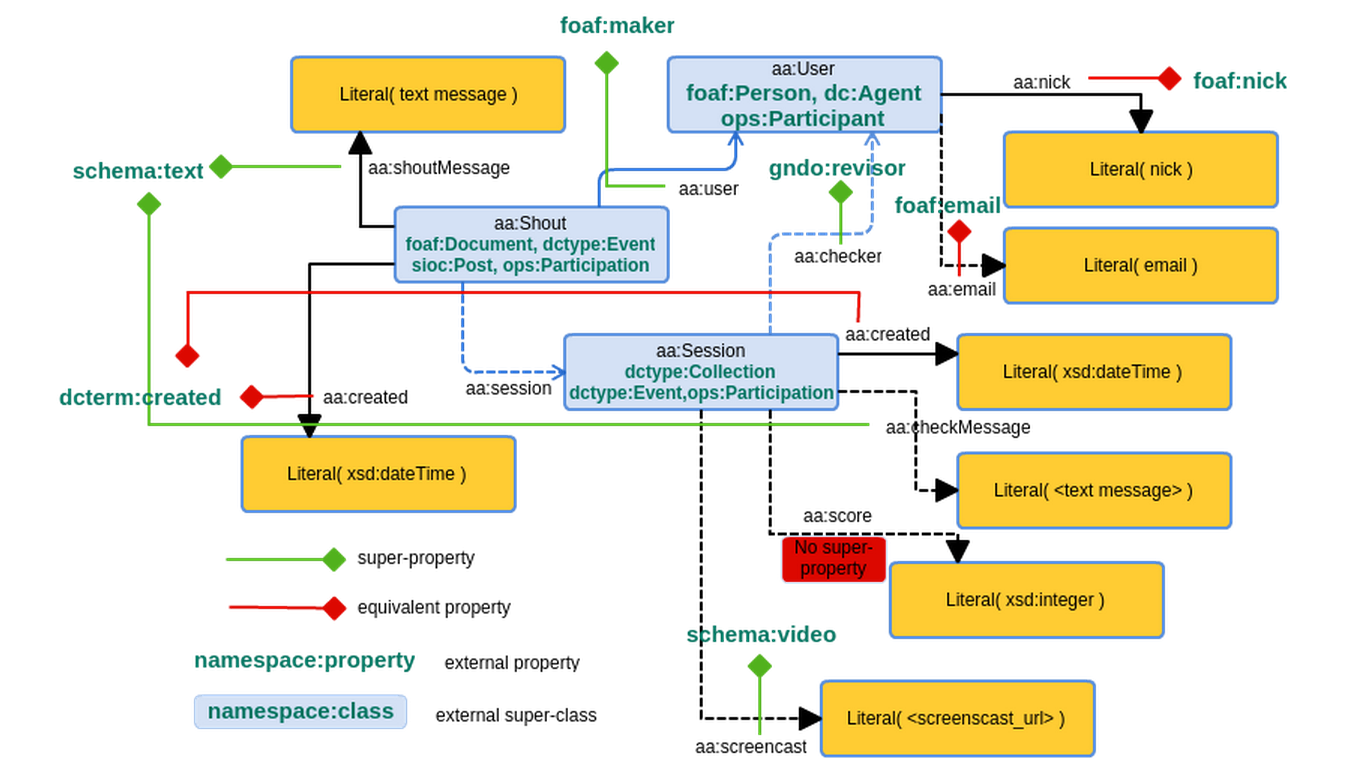
\includegraphics[width=1.5\textwidth]{imgs/ontologiaa_}
    \caption{The \ontologiaa: an \owl\ ontology of \aab. Classes are concepts related by properties. Classes are also related to upper ontologies (\foaf, \dc, \schema, \sioc, \gndo, \ops), as are properties. All properties are functional. Properties with a full line yield existential restrictions to the subjects of the triples suggested by the diagram: {\tt aa:user}, {\tt aa:nick}, {\tt aa:shoutMessage}, {\tt aa:created}. Blue lines mark object properties, while black lines are for data properties. All properties are functional, except for {\tt aa:nick} and {\tt aa:email}. For further information, see Section~\ref{sec:ont}.}.
    \label{fig:ontologiaa}
\end{figure}


\subsection{\rdfi\ data}
The \aab\ data is currently in relational and \nosql\ databases, and social networks messages to be mined (Section~\ref{sec:sofsup}). By using the same ontological background (see \ontologiaa\ in Section~\ref{sec:ont}), these data can be translated to \rdf\ for integration and linkage.

Script at~\cite{mysqlTri} outputs \rdf\ from a \mysql\ database, mostly from first \aab\ version.
Script at~\cite{mongoTri} transcribes a \mongodb\ database, mostly from \aab\ 0.1, to \rdf\ data.
Script at~\cite{ircTri} transcribes a shouts from \irc\ logs, mostly from first \aab\ version, to \rdf\ data.



\subsection{Linkage to external data}
The usage of \rdf\ and \owl\ protocols enables linked data facilities. \ontologiaai\ (and thus all \aab\ data) is integrated in two instances of special interest:
\begin{itemize}
    \item Through \ops, \aab\ data is linked to \opa, \obs, \vbs, and \ocd. These are Brazilian ontologies, with social participation focus, that has been used for data representation and conceptual studies~\cite{pnud5}.
    \item Through all other ontologies (e.g. \foaf, \dc, \schema, \sioc), \aab\ data is linked to relevant portions of the Giant Global Graph (\ggg) of Linked Open Data (\lod)~\cite{LOD}.
\end{itemize}

Gives meaning to data while easing data discovery and comparative analysis, to point a few of the advantages of such an approach~\cite{linkedDataBook}.

\section{Statistics}\label{sec:stats}
%\addcontentsline{toc}{section}{Data statistics}
\subsection{Occurrent activity}

\begin{table}[!h]
  \centering
  \caption{Registered \aab messages. Operational messages, for signaling session start, stop and publishing local logs (push) are the least abundant. Usage messages with quasi-null semantic content delivers indicative that the user is connected to \aab, but no more than that. Messages registering user processes were found to be 34770+1654 = 36424. There were 7504 \irc\ \aab\ messages, of which 1654 were not registered in databases, probably because of software failures. Automated messages of `lost timeslot' are the most numerous, with almost half of all messages. }\label{tab:msgTy}
  \begin{tabular}{|l|l|l|}\hline
      {\bf message content } & {\bf count} & {\bf type}   \\\hline\hline
 push & 1718 & \multirow{3}{*}{operational messages = 3936 } \\ 
start & 1169 & \\ 
 stop & 1049 & \\ \hline\hline
 empty shouts & 92    & \multirow{3}{*}{void messages = 17125} \\
 empty alerts & 83        &  \\
       notify & 16950     &  \\ \hline\hline
      message shouts & 34770 & \multirow{2}{*}{messages about ongoing tasks = 36424}  \\ 
      \irc\ message shouts & 1654 & \\ \hline
      lost timeslot & 59863 & client automated message \\ \hline\hline
      {\bf total} & 115694 & all messages are textual \\\hline
  \end{tabular}
\end{table}


\begin{table}[!h]
  \centering
  \caption{Registered \aab sessions.}\label{tab:session}
  \begin{tabular}{|l|l|}\hline
      {\bf description} & {\bf value}   \\\hline\hline
      number of sessions & 7288 \\ \hline
      number of shouts in sessions & 20299 \\ \hline
      number sessions with more than 1 shout & 905 \\ \hline
      number of shouts in sessions with more than 1 shout & 13916 \\ \hline
      number of users in sessions & 14 \\ \hline
      number of checkers in sessions & 36 \\ \hline
      number of screencasts in sessions & 295 \\ \hline
      number of scored sessions & 191 \\ \hline
      average session score & 3.18 \\ \hline
      standard deviation of score & 0.74 \\ \hline
      average number of shouts per session & 15.38 \\ \hline
      standard deviation of number of shouts & 19.82 \\ \hline
      first session from & 2011-07-06T03:23:05 \\ \hline
      last session from & 2014-04-01T09:11:36 \\ \hline

  \end{tabular}
\end{table}

% medida de atividade nos segundos, minutos, horas, dias da semana e do mes. Meses do ano.

\subsubsection{Time activity}

\begin{figure}[H]
    \hspace{-25mm}
    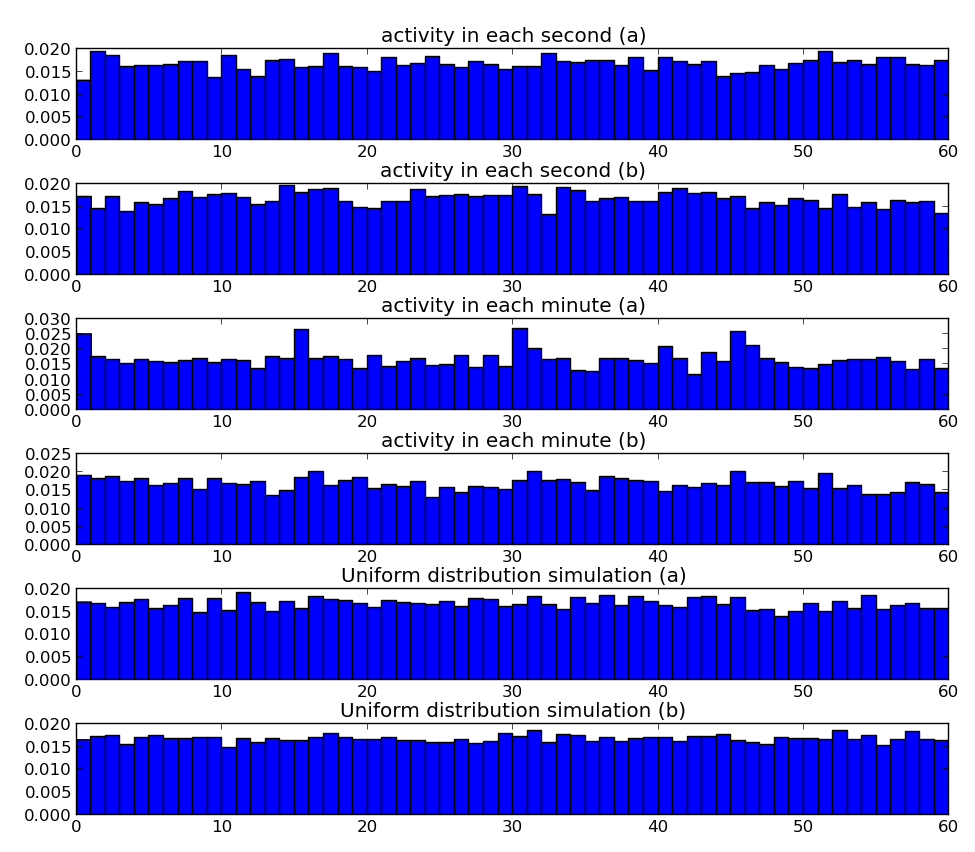
\includegraphics[width=1.3\textwidth]{imgs/segMinHist}
    \caption{\small Histogram of \aab\ activity along seconds and minutes. A strong 15 minutes pattern is visible in (a). The same pattern is apparent in all present histograms, although less incisive. This pattern was not found in mailing lists~\cite{rc1}, where distribution of activity along seconds and minutes was more homogeneous than Numpy uniform distribution simulator. In \aab\ the scene is the opposite: while simulations delivers $\tau=\frac{max[count(i)]}{min[count(i)]}\approx1.38$(a) and $\approx 1.26$ (b), shouts present $\tau=1.47$ and $\tau=1.48$, seconds for (a) and (b), and$\tau=2.32$ and $\tau=1.58$, minutes for (a) and (b). Means are considerably bellow $29.5$, which might indicate a tendency to shout messages in the beginning of minutes and hours. As these fluctuations among seconds and minutes were not observed in email lists (or other networks, as far as authors know), a hypothesis arises: the tasks at hand and the culture and socioeconomic factors makes timing more prominent. \aai\ itself is time-focused. Set (a) consists of all 15,145 messages from July, 2011 until December, 2011. Set (b) consists of all 21,055 messages from January, 2012 until January, 2015.}\label{fig:histSecMin}
\end{figure}


\begin{figure}[H]
    \hspace{-25mm}
    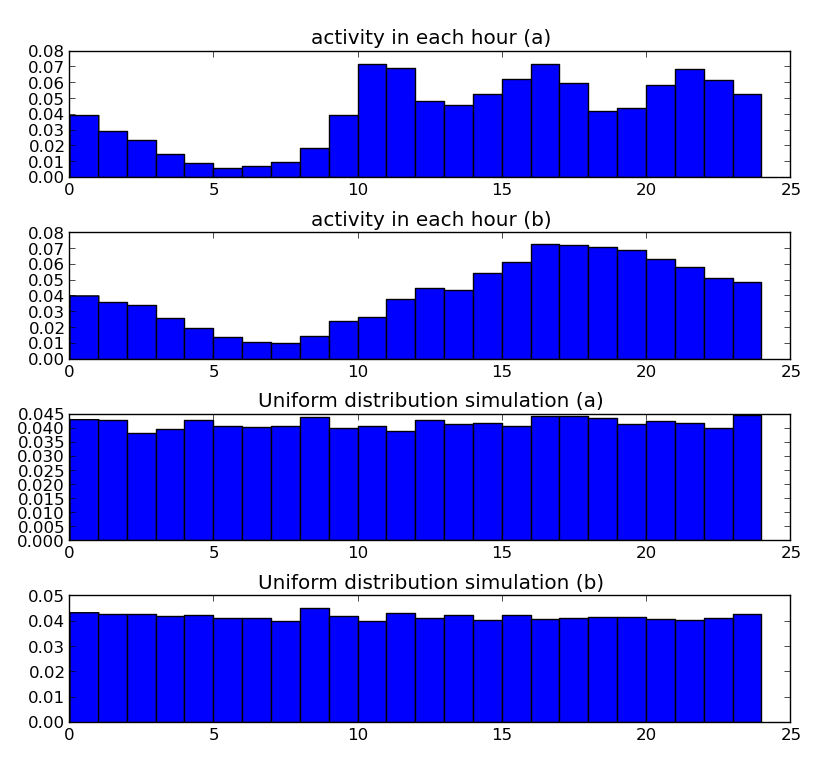
\includegraphics[width=1.3\textwidth]{imgs/hourHist}
    \caption{\small Histogram of \aab\ activity along hours of the day. Discrepancies in extreme incidences are more pronounced than observed with simulation using uniform distributions. While simulations delivers $\tau=\frac{max[count(i)]}{min[count(i)]}\approx1.18$(a) and $\approx 1.16$ (b), shouts present $\tau=13.5$ and $\tau=7.16$, respectively. Set (a) consists of all 15,145 messages from July, 2011 until December, 2011. Set (b) consists of all 21,055 messages from January, 2012 until January, 2015. Context (a) is in accordance with results driven from email lists~\cite{rc1}, where the activity peak is just before midday, and the second 12h period is the most active. Context (b) exhibits a very odd pattern, in which a climax is reached at 16h in a somewhat smooth progression.}\label{fig:histHour}
\end{figure}

\begin{figure}[H]
    \hspace{-25mm}
    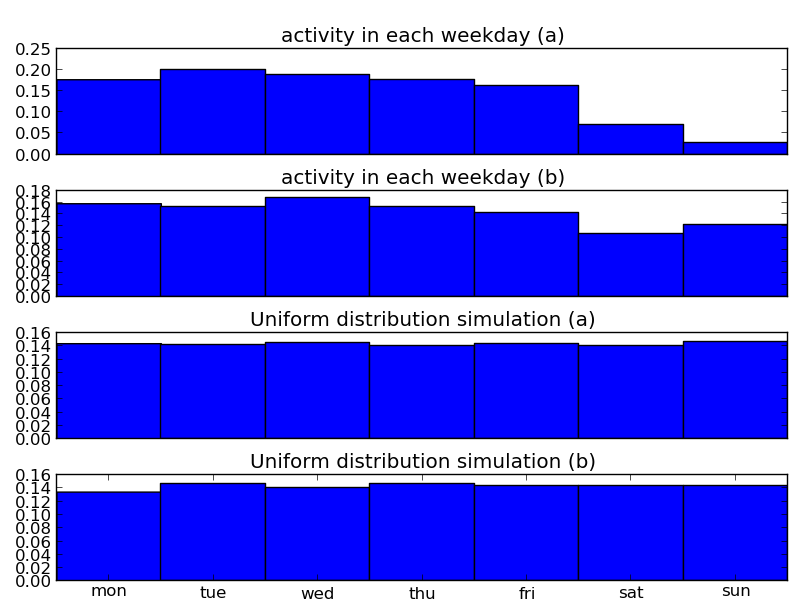
\includegraphics[width=1.3\textwidth]{imgs/weekdayHist}
    \caption{\small Histogram of \aab\ activity along days of the week. Discrepancies in extreme incidences are more pronounced than observed with simulation using uniform distributions. While simulations delivers $\tau=\frac{max[count(i)]}{min[count(i)]}\approx1.06$(a) and $\approx 1.07$ (b), shouts present $\tau=7.28$ and $\tau=1.57$, respectively. Set (a) consists of all 15,145 messages from July, 2011 until December, 2011. Set (b) consists of all 21,055 messages from January, 2012 until January, 2015. Context (a) exhibits a drop of more than half the activity on weekend days. This is more accentuated than results driven from email lists~\cite{rc1}, where weekends present about half the activity of other days. Context (b), on the other hand, has a drop of activity on weekends, but maintain levels above 50\%.}\label{fig:histWeekday}
\end{figure}

\begin{figure}[H]
    \hspace{-25mm}
    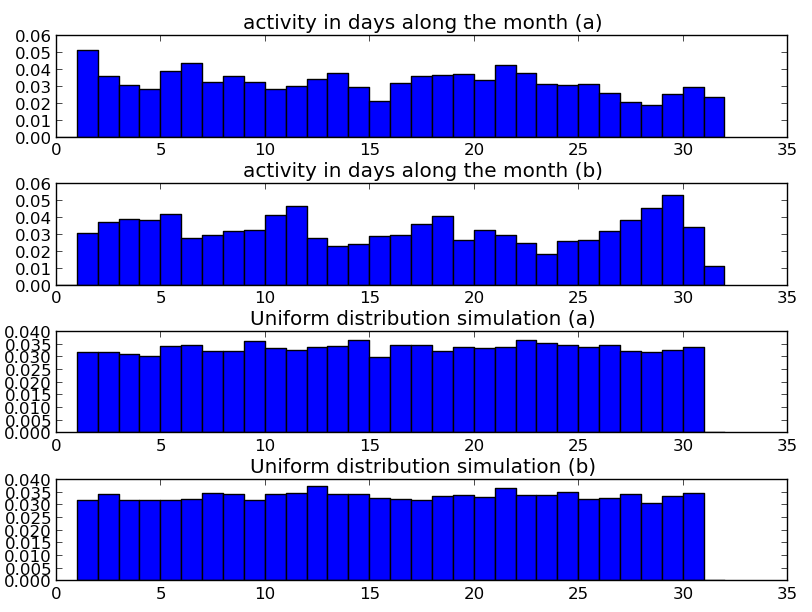
\includegraphics[width=1.3\textwidth]{imgs/monthdayHist}
    \caption{\small Histogram of \aab\ activity along days of the month. Discrepancies in extreme incidences are more pronounced than observed with simulation using uniform distributions. While simulations delivers $\tau=\frac{max[count(i)]}{min[count(i)]}\approx2.22$(a) and $\approx 2.23$ (b), shouts present $\tau=2.86$ and $\tau=4.75$, respectively. Set (a) consists of all 15,145 messages from July, 2011 until December, 2011. Set (b) consists of all 21,055 messages from January, 2012 until January, 2015. Context (a) seem to be shifted by 1 day if compared to context (b). Context (b) presents a 7 day periodicity until day $\approx 20$, where it seems extended until day 30. There is interesting to observe that although no hypothesis for this pattern was raised by authors, both months and weeks present patterns, while weekdays have no correlation with days of the month.}\label{fig:histDay}
\end{figure}



\begin{figure}[H]
    \hspace{-25mm}
    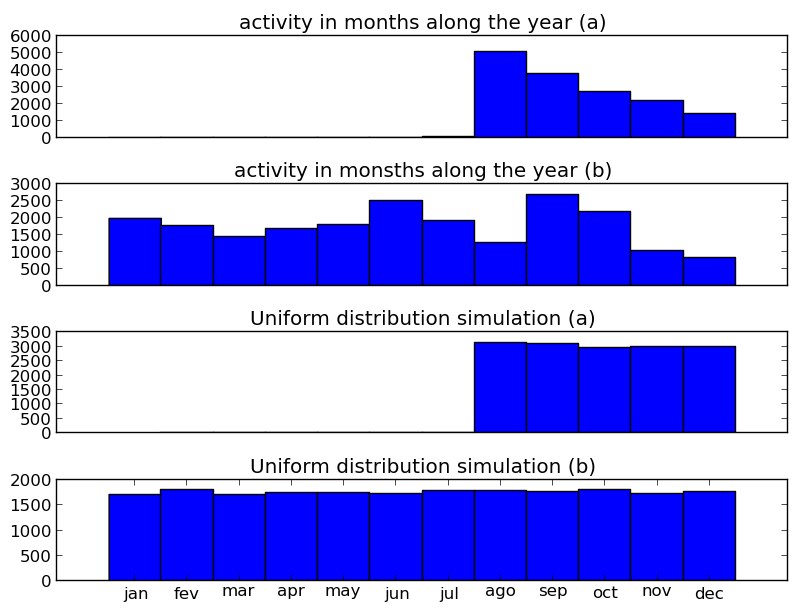
\includegraphics[width=1.3\textwidth]{imgs/monthsHist}
    \caption{\small Histogram of \aab\ activity along months of the year. Discrepancies in extreme incidences are more pronounced than observed with simulation using uniform distributions. While simulations delivers $\tau=\frac{max[count(i)]}{min[count(i)]}\approx1.06$(a) and $\approx 1.09$ (b), shouts present $\tau=3.71$ and $\tau=2.15$, respectively. Set (a) consists of all 15,145 messages from July, 2011 until December, 2011. Set (b) consists of all 21,055 messages from January, 2012 until January, 2015. Last months of the year are progressively less active. Activity seems to peak at the start of each quadrimester.}\label{fig:histMonth}
\end{figure}


\begin{figure}[H]
    \hspace{-25mm}
    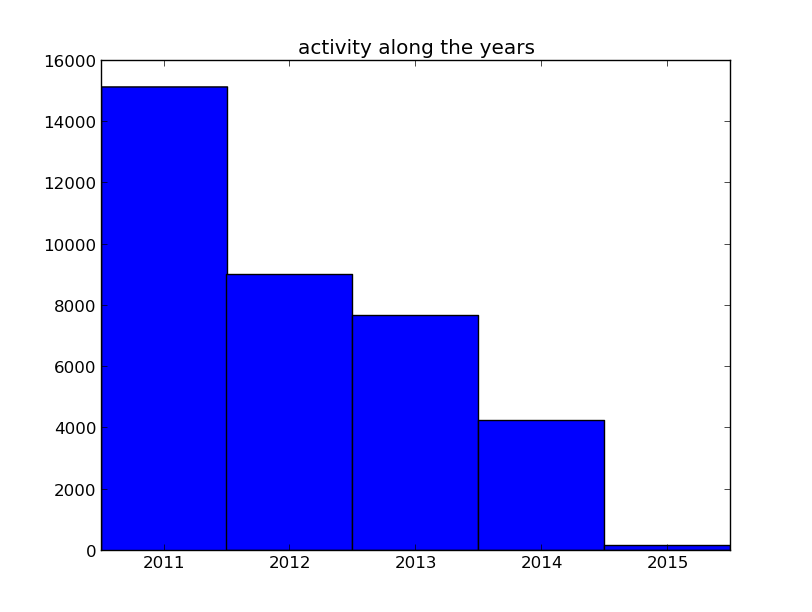
\includegraphics[width=1.3\textwidth]{imgs/yearHist}
    \caption{\small Histogram of \aab\ activity along the years. Activity was most pronounced at first 6 months. Less pronounced in 2014, where there was 2 months without \aab\ software support (see Section~\ref{sec:sofsup}). Only first days messages are considered from 2015, as it is when the writing started.}\label{fig:histMonth}
\end{figure}

\begin{figure}[H]
    \hspace{-25mm}
    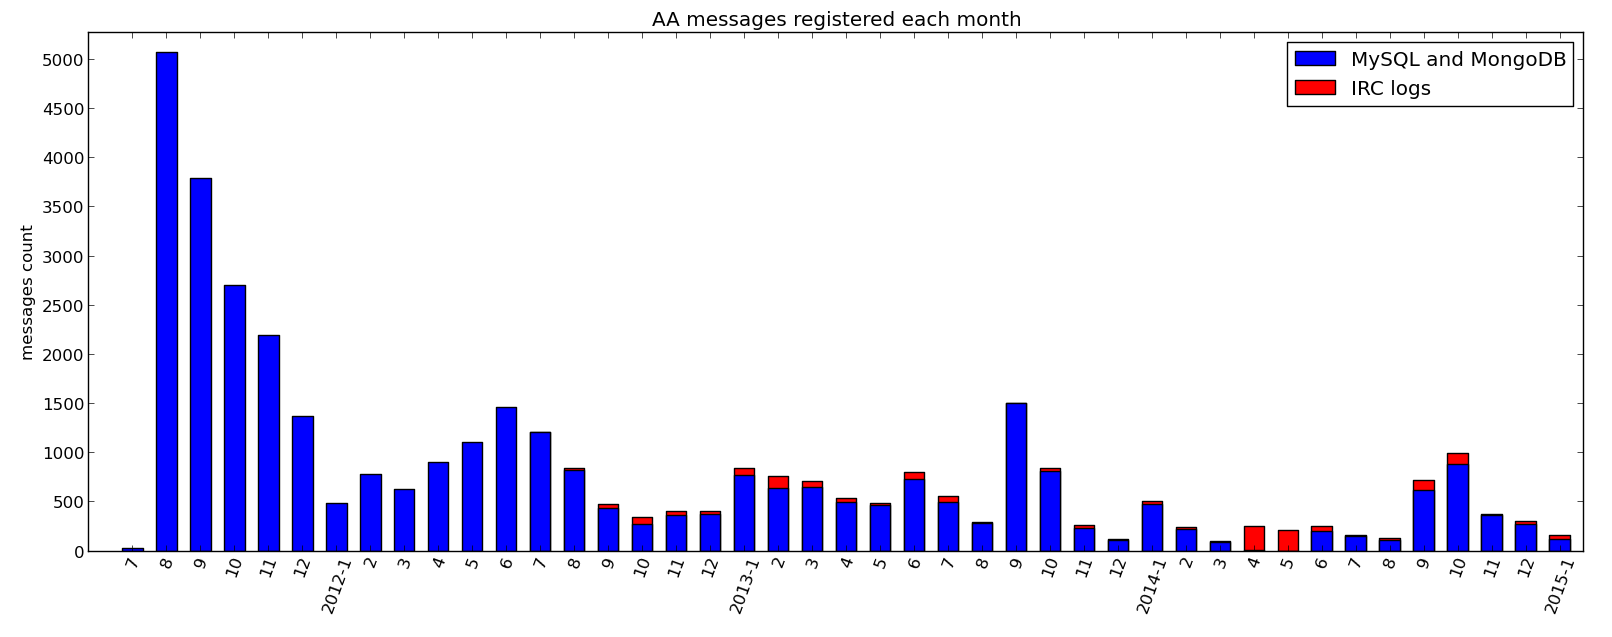
\includegraphics[width=1.3\textwidth]{imgs/actHist}
  \caption{\small The average number of messages each month is $\mu=507.1$, with a standard deviation of $\sigma=336.63 $.}\label{fig:mAct}
\end{figure}

\subsubsection{User activity}
\begin{figure}[H]
    \hspace{-25mm}
    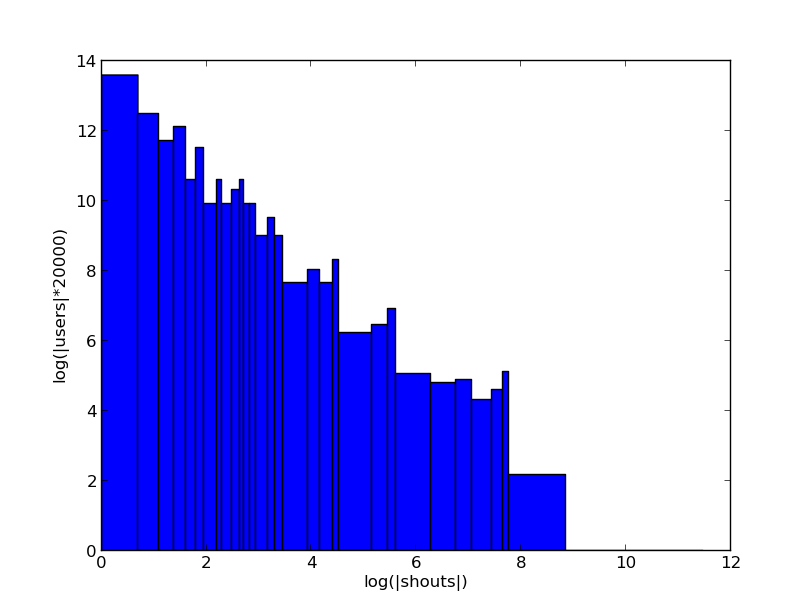
\includegraphics[width=1.3\textwidth]{imgs/userHist}
  \caption{\small Histogram of user activity. The free-scale trace can be noticed by the descending line in the log x log plot.}\label{fig:uH}
\end{figure}

Most active user (v1z) is responsible for 22.53\% of all activity and the two most active users (v1z, o0o0o) sum up to 42.40\%. The eight most active users (v1z, o0o0o, humannoise, mquasar, hick209, lari, Flecha, Fefo) sum 78.17\% of activity, while 95 less active users sum 11.84\%. These are in accordance with natural observations, as is the free-scale trace in Figure~\ref{fig:uH}. Total number of users are 106, while (valid) messages sum 36,424.

\subsubsection{Character and token incidence}
\begin{figure}[H]
    \hspace{-25mm}
    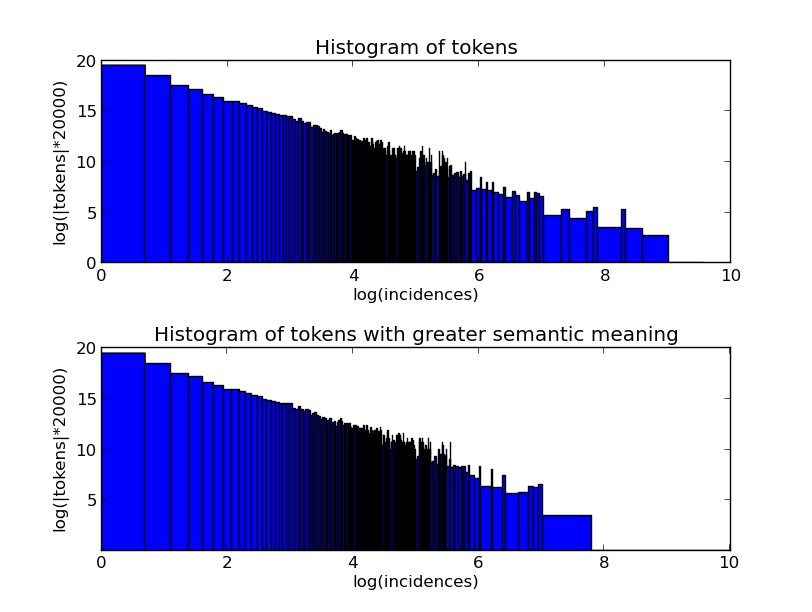
\includegraphics[width=1.3\textwidth]{imgs/tokenHist}
  \caption{\small Histogram of token incidence in the logarithmic scale: (a) all tokens, (b) tokens which are not a English or Portuguese stopwords, \url s or punctuations. The Pareto trace can be noticed by the descending line in the log x log plot. Noteworthy is that theory predicts histogram (b) to exhibit a line in the logarithmic scale, but histogram (a) follows predictions more closely.}\label{fig:tH}
\end{figure}

\begin{figure}[H]
    \hspace{-25mm}
    \includegraphics[width=1.3\textwidth]{imgs/diffHist}
  \caption{\small Histogram of incident and existent token size in number of characters. Top histogram considers all tokens; mean token size of incident tokens is $\mu_{in}=5.74$; standard deviation $\sigma_{in}=5.9$; mean token size of existent tokens is $\mu_{ex}=$; standard deviation $\sigma_{ex}=$. Middle histogram considers tokens which are not punctuations, \url s or stopwords (Portuguese and English); $\mu_{in}=6.79$, $\sigma_{in}=4.70$, $\mu_{ex}=7.95$, $\sigma_{ex}=5.00$. Bottom histogram considers all radicals from tokens used for middle histogram; $\mu_{in}=5.57$, $\sigma_{in}=5.02$, $\mu_{ex}=7.89$, $\sigma_{ex}=7.59$.}\label{fig:dH}
\end{figure}



\begin{table}[!h]
%  \centering
    \hspace{-25mm}
  \caption{Further observations on tokens. }\label{tab:msgTy}
  \begin{tabular}{|l|p{11cm}|}\hline
      {\bf description } & {\bf incidence }  \\\hline\hline
30 most incident words & ('codigo', 346), ('pouco', 347), ('AA', 355), ('paper', 357), ('dando', 379), ('wiki', 391), ('email', 413), ('escrevendo', 421), ('q', 423), ('terminando', 466), ('scilab', 497), ('p', 508), ('/Users/rfabbri/lib/notas/todos:', 511), ('eh', 541), ('aa', 596), ('ver', 613), ('indo', 620), ('lendo', 711), ('vou', 772), ('fazendo', 795), ('vendo', 906), ('fazer', 960), ('tentando', 977), ('agora', 1000), ('pra', 1058), ('nao', 1075), ('ainda', 1118), ('sobre', 1605), ('commit', 2472), ('git', 2535)  \\ \hline
30 most incident radicals & ('volt', 458), ('feit', 490), ('arrum', 506), ('p', 508), ('/users/rfabbri/lib/notas/todos:', 511), ('trabalh', 513), ('scilab', 540), ('eh', 546), ('nov', 580), ('algum', 589), ('escrev', 603), ('ver', 616), ('ind', 651), ('ach', 708), ('email', 741), ('lend', 858), ('test', 929), ('vou', 956), ('aa', 974), ('vend', 986), ('agor', 1080), ('pra', 1086), ('nao', 1114), ('aind', 1206), ('termin', 1274), ('tent', 1335), ('sobr', 1611), ('faz', 1882), ('git', 2544), ('commit', 2579)  \\ \hline
number of web addresses & 1431 \\\hline

  \end{tabular}
\end{table}



\subsubsection{Morphosyntactic incidence}
\subsection{Dependent activity}
\subsubsection{Time and user dependent activity}
\subsubsection{Language and user dependent activity}
\subsubsection{Language and time dependent activity}
\subsubsection{Time-related stability}
\subsection{Network activity}
\subsubsection{Time user networks}
% ambito no pico de atividade relaciona usuarios
% rede unipartida de usuarios relacionados

\subsubsection{Lexical user networks}
% utilização de verbetes em comum relaciona usuarios
% rede unipartida de usuarios relacionados

\subsubsection{Network measures}
% tabela com grausm forcas, clustering, betweenness, etc.

\subsubsection{Network primitive sectioning}
% diferenciação no particionamento das diferentes redes.

\subsection{Principal components formation}
\subsection{Immediate clustering}
\subsubsection{Users clustering}
% cada usuario eh um individuo
\subsubsection{Words clustering}
% cada verbete eh um individuo
\subsection{Timeslot clustering}
% cada hora do dia eh um individuo
\subsection{Comparative analysis}
\subsection{\aai, \ocd, and \participa}

\section{Results}\label{sec:res}
Although a weak evidence, the closer fit to natural predictions of using all tokens, including \url s and punctuations, instead of only a canonical set of words, raises the hypothesis that these elements are shares some levels of meaning with ordinary words, at least in virtual environments.

\section{Conclusions}\label{sec:con}
\subsection{Further work}
\subsection{Acknowledgments}
Vilson pelas versoes iniciais do aa e do plugin da lalenia.
karmiac e bzum e andres pelo aa.
Ricardo Fabbri pelo artigo
Marcos Mendoça pelo paainel.
Felipe Machado, por atribuir a responsabilidade de erigir um sistema de co-working nos idos tempos de 2009.
Criadores do supy, django python, numpy e outras ferramentas de mineracao


%\addcontentsline{toc}{subsection}{\ontologiaa: the \aab\ ontology}
%\begin{wrapfigure}{l}{0.4\textwidth} % Inline image example
%\begin{center}
%\includegraphics[width=0.38\textwidth]{telao1.png}
%\end{center}
%\caption{\small Telão para streaming de estruturas sociais, usado no \#arenaNETmundial, \#ocupaGOV e outras ocasiões. Tela com rede de retweets e relacionamento via hashtag e vocabulário. Atualizada a cada 10 segundos com os relacionamentos implicados pelos dos tweets mais recentes.}\label{fig:telao}
%\end{wrapfigure}

%\begin{figure}[H]
%  \centering
%    \includegraphics[width=.7\textwidth]{telao2.png}
%  \caption{\small Telão para streaming de estruturas sociais, usado no \#arenaNETmundial, \#ocupaGOV e outras ocasiões. Tela com relacionamentos de hashtags e vocabulário. Atualizada a cada 10 segundos com conteúdo dos tweets mais recentes.}\label{fig:telao2}
%\end{figure}










%----------------------------------------------------------------------------------------
%   BIBLIOGRAPHY
%----------------------------------------------------------------------------------------

%\bibliographystyle{unsrt}
%\bibliographystyle{plain}
\bibliographystyle{ieeetr}
\bibliography{ensaio}

%----------------------------------------------------------------------------------------

\end{document}
